\documentclass[11pt]{article}
\usepackage[margin=1in]{geometry}
\usepackage{volfit_preamble}
\graphicspath{{figures/}}

\title{\textbf{Beyond the Last Quote}\\[2pt]
\large What a fitter can prove, must choose, and has to police in the
wings\\[2pt]
\normalsize Vol-Fitter Technical Notes, No.~09}
\author{Vol-Fitter}
\date{\today}

% Note-local notation (shared symbols come from volfit_preamble).
\newcommand{\bL}{\beta_L}
\newcommand{\bR}{\beta_R}
\newcommand{\AL}{A_L}
\newcommand{\AR}{A_R}

\begin{document}
\maketitle

% Generated numbers.  wings_lastquote_tables.tex carries everything unique
% to this edition (gen_wings_lastquote.py).  Never retype a generated number.
% Auto-generated by gen_wings_lastquote.py — do not edit.
\newcommand{\wlqherobetaL}{0.422}
\newcommand{\wlqherobetaR}{0.054}
\newcommand{\wlqheroqstar}{0.74}
\newcommand{\wlqheroextrapshare}{48}
\newcommand{\wlqbetaLQDL}{0.0971}
\newcommand{\wlqbetaLQDR}{0.0358}
\newcommand{\wlqbetaSVIL}{0.1093}
\newcommand{\wlqbetaSVIR}{0.0364}
\newcommand{\wlqbetaMCSL}{0.1057}
\newcommand{\wlqbetaMCSR}{0.0297}
\newcommand{\wlqsvicap}{0.1093}
\newcommand{\wlqhatslopediff}{\ensuremath{1.0\times10^{-17}}}
\newcommand{\wlqhatgdent}{-2.0}
\newcommand{\wlqhatzmin}{-2.8}
\newcommand{\wlqhatbasegmin}{0.14}
\newcommand{\wlqarbgraw}{-8.8}
\newcommand{\wlqarbgfixed}{-0.027}
\newcommand{\wlqbyteid}{\ensuremath{1.3\times10^{-13}}}
\newcommand{\wlqphantominside}{0.0}
\newcommand{\wlqphantomwide}{142.0}
\newcommand{\wlqlvswingbp}{284}
\newcommand{\wlqnaivepsi}{-6.0}
\newcommand{\wlqstablepsi}{0.0}
\newcommand{\wlqrefagree}{\ensuremath{1.0\times10^{-17}}}
\newcommand{\wlqgencommit}{f8562c1}
\newcommand{\wlqgendate}{2026-07-18}


\begin{abstract}
On a live SPY surface, \wlqheroextrapshare\% of the strike range the
application draws lies beyond the quoted board: no quote constrains it,
no fit error reports it, and yet the var-swap pairing of Note~08, every
tail risk metric, and the graph extrapolator of Note~14 all integrate
straight through it.  This lecture organizes the wing treatment shared by
the four smile models around a three-way division of epistemic labour.
What can be \emph{proved}: model-free asymptotics --- the total-variance
wing slope of any arbitrage-free smile obeys $\beta\le2$ (derived here
from first principles: along a steeper ray the far-OTM call refuses to
become worthless), and Lee's moment formula $\beta=\psi(p)$ ties the
slope to the tail's critical moment exponent.  What must be \emph{chosen}:
inside that cone the quotes cannot select --- the three parametric models
fitted to one window print slopes $(\wlqbetaLQDL,\wlqbetaSVIL,
\wlqbetaMCSL)$ on the put side by three different mechanisms (structural,
soft-capped, inherited), and the local-vol deep-put slope moves a
two-year fair var-swap strike by \wlqlvswingbp\ vol bp --- each wing is a
stated contract, not an estimate.  What has to be \emph{policed}: the
limit is not the wing --- a hat whose realized slope perturbation
measures below $10^{-16}$ still drives the Durrleman density to
$g=\wlqhatgdent$ at $z=\wlqhatzmin$, so finite-range admissibility needs
its own machinery: the census-guided put-wing hinge (worst $g$
$\wlqarbgraw\to\wlqarbgfixed$ on the synthetic arb slice, byte-identical
to \wlqbyteid\ on a clean one, validated by the input/output ablation of
the case file), and the \emph{confinement principle} deciding where each
constraint has jurisdiction --- a two-curve constraint sampled in the
extrapolated region manufactures a \wlqphantomwide-variance-bp phantom
violation between two fictions, while the same constraint confined to
the traded range sees exactly none.
\end{abstract}

\newpage
\tableofcontents
\newpage

%======================================================================
\section{The last quote}
\label{sec:problem}

\Cref{fig:hero} is a production exhibit: the longest SPY expiry from a
live surface, with \wlqheroextrapshare\%\footnote{Share of the drawn
strike range outside the prepared quotes; the drawing range itself is a
display choice --- see \cref{sec:limits}.} of its drawn strike range
beyond the last quote.  Nobody quotes the far wings, yet everything
downstream reads them: the var-swap replication integrates
$1/K^{2}$-weighted prices into the tails (Note~08's pairing loads
\emph{exactly} on this region), risk metrics difference the wings, and
the graph extrapolator (Note~14) inherits whatever tail the fitted model
draws.  Wing errors are invisible in the fit RMS --- there are no quotes
to miss --- and surface later as a mispriced tail somewhere else.

\begin{figure}[H]
\centering
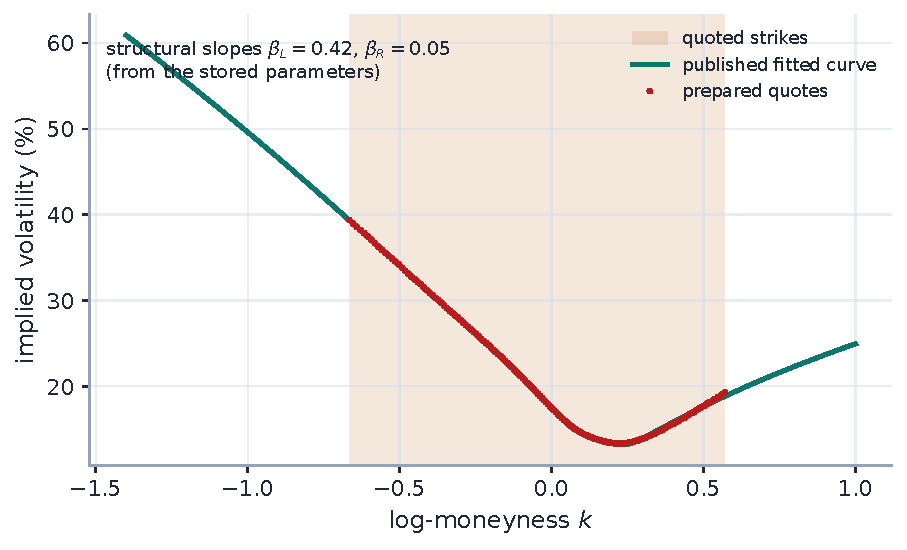
\includegraphics[width=0.88\textwidth]{fig_wlq_hero.pdf}
\caption{The production problem, on a live SPY expiry (2027-06,
Massive feed).  The prepared quotes (dots) span the shaded band;
\wlqheroextrapshare\% of the drawn curve is extrapolation.  The wing the
application draws there is not an estimate --- it is the model's stated
law, with structural Lee slopes $\bL=\wlqherobetaL$, $\bR=\wlqherobetaR$
computed from the stored slice parameters.}
\label{fig:hero}
\end{figure}

Two different things can go wrong out there, and the whole note turns on
keeping them distinct.  The \emph{asymptotic} slope of total implied
variance can violate a model-free bound --- an arbitrage against the
existence of any terminal law at all (\cref{sec:prove}).  And the
\emph{finite} wing can lose density positivity even with perfectly
admissible slopes --- a butterfly arbitrage parked in the extrapolated
region where no quote objects (\cref{sec:police}).  The first failure is
excluded by theorems; the second only by machinery.  Between the two
sits a region the mathematics deliberately leaves open: within the
admissible cone, the data cannot choose the wing, so the model must
(\cref{sec:choose}).

\begin{invariant}
\begin{enumerate}[leftmargin=1.6em]
\item Every displayed wing is Lee-admissible: $\beta\le2$, structurally
where possible, by a soft cap otherwise.
\item Single-slice (butterfly) constraints \emph{extend} into the wings;
two-slice (calendar) constraints are \emph{confined} to the traded range
(\cref{sec:confine}).
\item Every wing guard is strictly additive: on an already-clean slice it
is byte-identical to no guard.
\item The tail is a property of the model's extrapolation law, not of
the quotes; where the desk needs control (the local-vol deep puts) the
slope is an explicit knob, and a calibrated variable exactly when an
instrument exists that observes it.
\end{enumerate}
\end{invariant}

\paragraph{Conventions and the notation ledger.}
$T$ is the expiry; $t$ appears only as the local-vol running clock.
Subscripted $\partial$ for all derivatives; no primes.  One vol bp is
$10^{-4}$ of absolute volatility; a variance bp is $10^{-4}$ of total
variance.

\begin{table}[H]
\centering\footnotesize
\setlength{\tabcolsep}{3pt}
\begin{tabular}{@{}llll@{}}
\toprule
$k,\ K=e^{k},\ F=1$ & log-moneyness; strike; forward &
$\tvar(k),\ \Black(k,\tvar)$ & total implied variance; Black call\\[2pt]
$\bL,\ \bR$ & wing slopes $\limsup \tvar/|k|$ &
$p,\ q,\ \psi$ & moment exponents; the Lee map\\[2pt]
$\AL,\ \AR$ & LQD endpoint tail scales &
$z,\ v(z),\ \sigma_{\mathrm{ref}}$ & standardized moneyness; variance; scale\\[2pt]
$g(z)$ & Durrleman density factor &
$\alpha,\ c,\ h,\ \kappa$ & a hat's amplitude, centre, width, decay\\[2pt]
$\locvar(t,x),\ a$ & local variance; left-slope multiplier &
$\lambda$ & penalty weights\\
\bottomrule
\end{tabular}
\caption{Every symbol in the note.  $p$ and $q$ are always moment
exponents (never model parameters); the SVI wing formulas use only
$b,\rho$.}
\label{tab:ledger}
\end{table}

%======================================================================
\section{What can be proved: the admissible cone}
\label{sec:prove}

Extrapolation begins where estimation ends, so start with what holds
with \emph{no} data at all.  Let $\tvar(k,T)$ be total implied variance
and define the wing slopes
\[
\bR=\limsup_{k\to+\infty}\frac{\tvar(k,T)}{k},\qquad
\bL=\limsup_{k\to-\infty}\frac{\tvar(k,T)}{|k|} .
\]

\subsection{The ceiling, from first principles}

\begin{proposition}[The model-free ceiling]
\label{prop:ceiling}
For any arbitrage-free smile, $\bL,\bR\le2$.
\end{proposition}

\begin{proof}
Take the right wing.  Because the terminal law has a finite mean
($\E[S_T]=1$), dominated convergence forces the OTM call to become
worthless: $C(k)=\E[(S_T-e^{k})^{+}]\to0$ as $k\to\infty$.  Now compute
what the Black functional does along a ray $\tvar=\beta k$.  Its
arguments are
\[
d_{\pm}=-\frac{k}{\sqrt{\tvar}}\pm\frac{\sqrt{\tvar}}{2}
=\sqrt{k}\Big(\mp\frac{1}{\sqrt\beta}\pm\frac{\sqrt\beta}{2}\Big)
\Big|_{\pm}
=\sqrt{k}\,\Big(\frac{\sqrt\beta}{2}-\frac{1}{\sqrt\beta}\Big)
\ \text{for } d_{+}.
\]
If $\beta>2$ then $\sqrt\beta/2>1/\sqrt\beta$, so $d_{+}\to+\infty$ and
$\Black(k,\beta k)=\PhiN(d_{+})-e^{k}\PhiN(d_{-})\to1$ (the second term
vanishes: $e^{k}\PhiN(d_{-})\sim e^{k}\phin(d_{-})/|d_{-}|$ and
$k+\ln\phin(d_{-})\to-\infty$ for $\beta>2$).  A smile with
$\tvar(k)\ge\beta k$ along a sequence $k\to\infty$ therefore prices
calls bounded away from zero at arbitrarily high strikes ---
contradicting $C(k)\to0$.  Monotonicity of $\Black$ in $\tvar$ converts
the ray statement into the $\limsup$ statement.  The left wing mirrors
through the put per unit of strike: $P(k)/e^{k}=\E[(1-S_T e^{-k})^{+}]
\to\Prob(S_T=0)$ as $k\to-\infty$, while along a ray of slope
$\beta>2$ the Black put forces $P(k)/e^{k}\to1$ --- the entire mass at
zero, impossible for a law with mean one.
\end{proof}

\Cref{fig:ceiling}B draws the proof: along rays $\tvar=\beta k$ the
production Black evaluator sends the call to $0$ for $\beta<2$ and to
$1$ for $\beta>2$.  The boundary ray $\beta=2$ pins the call at exactly
$\tfrac12$ --- also inconsistent with $C\to0$, which sharpens the
statement in a way worth a remark:

\begin{remark}[The ceiling is a supremum, not a member]
\label{rem:boundary}
$\bR=2$ is attainable as a $\limsup$ --- $\tvar(k)=2k-c\sqrt{k}$ type
wings approach the ceiling from below --- but the exact ray
$\tvar=2k$ is itself already inadmissible at large $k$.  A model that
caps its wing \emph{at} $2$ must therefore approach the cap, never sit
on it; the LQD guard below ($\AR<1$ strictly) is this remark in
production form.
\end{remark}

\subsection{Lee's moment formula}

The ceiling says how steep a wing \emph{cannot} be.  Lee's theorem says
exactly how steep it \emph{is}, in terms of the tail of the law:

\begin{theorem}[Lee \cite{Lee2004}]
\label{thm:lee}
Let $p^{*}=\sup\{p:\E[S_T^{1+p}]<\infty\}$ and
$q^{*}=\sup\{q:\E[S_T^{-q}]<\infty\}$.  Then
\begin{equation}
\boxed{\;\bR=\psi(p^{*}),\qquad \bL=\psi(q^{*}),\qquad
\psi(p)=2-4\big(\sqrt{p^{2}+p}-p\big)\in[0,2].\;}
\label{eq:psi}
\end{equation}
\end{theorem}

\begin{proof}[Proof sketch (the easy half)]
Suppose $\E[S_T^{1+p}]<\infty$.  From the elementary bound
$(s-K)^{+}\le c_p\,s^{1+p}K^{-p}$ with $c_p=p^{p}/(1+p)^{1+p}$
(maximize over $s$), $C(K)=O(K^{-p})$.  Matching this decay against the
Black asymptotics of a wing of slope $\beta$ --- the same $d_\pm$
computation as in \cref{prop:ceiling}, one order deeper --- shows the
call along a ray of slope $\beta$ decays like
$K^{-\big(\frac{1}{2\beta}+\frac{\beta}{8}-\frac12\big)}$ up to
algebraic factors; consistency forces
$\frac{1}{2\beta}+\frac{\beta}{8}-\frac12\ge p$, i.e.\
$\beta\le\psi(p)$.  Hence $\bR\le\psi(p)$ for every $p<p^{*}$.  The
converse --- that the $\limsup$ \emph{attains} $\psi(p^{*})$ --- is the
substance of \cite{Lee2004}; regular-variation refinements are in
\cite{BenaimFriz2009}.
\end{proof}

\begin{lemma}[Properties of the Lee map]
\label{lem:psi}
$\psi$ is a strictly decreasing bijection from $[0,\infty]$ onto
$[0,2]$, with $\psi(0)=2$, $\psi(\infty)=0$, and explicit inverse
$p=\tfrac{1}{2\beta}+\tfrac{\beta}{8}-\tfrac12$.
\end{lemma}

\begin{proof}
Write $\psi(p)=2\big(\sqrt{p+1}-\sqrt p\big)^{2}$: the parenthesis is
positive and strictly decreasing (derivative
$\half(1/\sqrt{p+1}-1/\sqrt p)<0$), with limits $1$ at $p=0$ and $0$ at
$\infty$.  Solving $\beta=2(\sqrt{p+1}-\sqrt p)^{2}$ for $p$ is
elementary algebra.
\end{proof}

\begin{figure}[H]
\centering
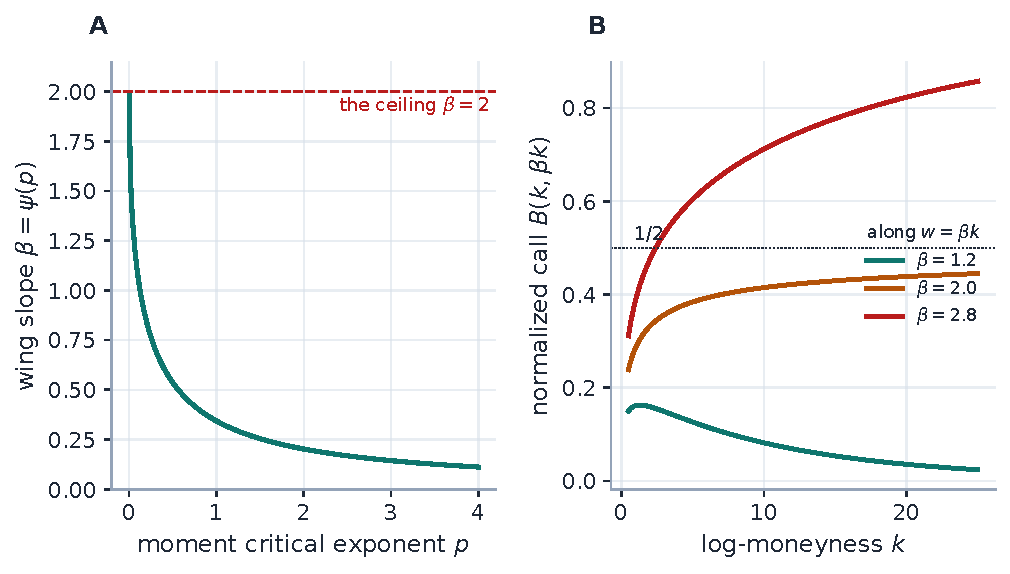
\includegraphics[width=\textwidth]{fig_wlq_ceiling.pdf}
\caption{What can be proved.  A: the Lee map $\beta=\psi(p)$ ---
heavier tails (smaller critical exponent) force steeper variance wings,
capped at the model-free ceiling.  B: the ceiling derived visually
(production Black evaluator): along rays $\tvar=\beta k$ the far-OTM
call dies for $\beta<2$, is pinned at $\tfrac12$ on the boundary ray,
and tends to $1$ for $\beta>2$ --- a smile that steep prices calls that
refuse to become worthless, which no terminal law can produce
(\cref{prop:ceiling}).}
\label{fig:ceiling}
\end{figure}

\begin{heuristic}
The wing slope and the tail heaviness are two faces of one coin.  A fat
right tail (few finite positive moments) \emph{must} show up as a steep
right variance wing; a model that draws a flat wing over a fat-tailed
density is internally inconsistent and will misprice far-OTM calls.
Lee's formula is not a nuisance constraint but a consistency condition
between the smile and the law it implies --- which is why the model
built from the law outward (LQD) satisfies it automatically, and the
models built from the smile outward (SVI, MCS) need a cap or a
diagnosis.
\end{heuristic}

\begin{remark}[Evaluating $\psi$ is itself a lesson]
\label{rem:naive}
The textbook form $\psi(p)=2-4(\sqrt{p^{2}+p}-p)$ subtracts two
$O(p)$ quantities whose difference is $O(1)$: catastrophic cancellation.
At $p=10^{16}$ it returns $\wlqnaivepsi$ --- outside the codomain
$[0,2]$ entirely --- while the algebraically identical
$\psi(p)=2-4/\big(\sqrt{1+1/p}+1\big)$ returns $\wlqstablepsi$, the
correct limit to double precision.  The production implementation uses
the stable form (\cref{app:ref}); extreme exponents are not academic ---
they arise whenever an endpoint scale underflows
(\cref{sec:choose}).
\end{remark}

%======================================================================
\section{What must be chosen: four wing contracts}
\label{sec:choose}

Everything inside the cone of \cref{sec:prove} is mathematically
admissible, and the quotes --- which end at the last strike --- cannot
select among admissible tails.  \Cref{fig:extrap} makes the
indeterminacy concrete: three parametric models fitted to the same
twenty-three quotes agree to vol bps inside the window and then each
draws its own wing.  That divergence is not a defect to be averaged
away: past the last quote a wing is a modelling \emph{choice}, and what
the fitter guarantees is not agreement but a stated, tested \emph{wing
contract} per model, with per-model teeth.  \Cref{tab:betas} collects
the fitted slopes; the four contracts follow.

\begin{figure}[H]
\centering
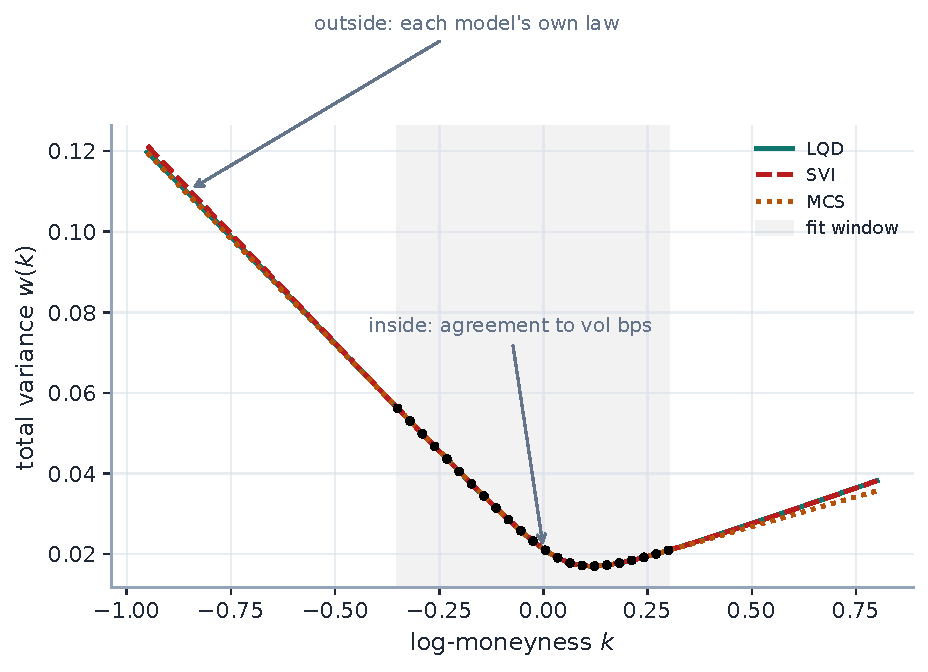
\includegraphics[width=0.86\textwidth]{fig_wlq_extrap.pdf}
\caption{What must be chosen.  Three models fitted to the same window
(shaded) agree to vol bps where quotes exist and then diverge --- each
tail is the property of \emph{its} extrapolation law, not of the
identical data.  All three are Lee-admissible; the data has no further
opinion.  Choosing a model \emph{is} choosing an extrapolation law.}
\label{fig:extrap}
\end{figure}

\begin{table}[H]
\centering
\caption{Analytic asymptotic wing slopes on the benchmark window (fresh
production fits); all far below the ceiling $2$.}
\label{tab:betas}
\begin{tabular}{lrrl}
\toprule
Model & $\bL$ (put) & $\bR$ (call) & mechanism\\
\midrule
LQD & \wlqbetaLQDL & \wlqbetaLQDR & structural via $\psi(1/A)$\\
SVI & \wlqbetaSVIL & \wlqbetaSVIR & linear $b(1\mp\rho)$, soft Lee cap\\
MCS & \wlqbetaMCSL & \wlqbetaMCSR & base wings, hats neutral
(\cref{prop:zerowing})\\
\bottomrule
\end{tabular}
\end{table}

\subsection{LQD: Lee-consistent by construction}

The LQD slice (Note~01) parametrizes the log quantile density with
logarithmic endpoints, which makes the return tails exactly
\emph{exponential} with scales $\AL,\AR$ read off the endpoint values of
the basis expansion.  The moment exponents follow in two lines: the
right tail of $X=\log S_T$ decays like $e^{-x/\AR}$, so
$\E[S_T^{1+p}]=\E[e^{(1+p)X}]$ converges iff $1+p<1/\AR$, giving
$p^{*}=1/\AR-1$; the left tail decays like $e^{x/\AL}$ as
$x\to-\infty$, so $\E[S_T^{-q}]=\E[e^{-qX}]$ converges iff $q<1/\AL$,
giving $q^{*}=1/\AL$.  By \cref{thm:lee},
\begin{equation}
\bL=\psi(1/\AL),\qquad \bR=\psi(1/\AR-1),\qquad \AR<1 .
\label{eq:lqd_wings}
\end{equation}
No penalty enforces this --- it is structural, the law-outward
construction of the Heuristic above.  The only wing constraint is the
hard $\AR<1$ (finite forward; the strict inequality is
\cref{rem:boundary} in action), held by Note~01's soft barrier.  The
guards of \cref{rem:naive} handle underflowed scales:
$\AR\ge1\mapsto\bR=2$, $A=0\mapsto\beta=0$.  The hero figure's slopes
$(\wlqherobetaL,\wlqherobetaR)$ are exactly \eqref{eq:lqd_wings}
evaluated on the stored production parameters.

\subsection{SVI: linear wings under a soft cap}

Raw SVI (Note~02) has exactly linear variance wings,
$\tvar(k)\sim b(1\mp\rho)|k|$, so $\bL=b(1-\rho)$ and $\bR=b(1+\rho)$
in closed form.  Lee's bound is then one explicit inequality,
$b(1+|\rho|)\le2$, enforced as a soft hinge
$\max\big(b(1+|\rho|)-\beta_{\max},0\big)$ at weight $10^{3}$ alongside
the min-variance penalty (cap default $2$).  On any admissible smile
both hinges are exactly zero --- they fence the optimizer out of the
inadmissible region without touching admissible fits; the benchmark fit
sits at $b(1+|\rho|)=\wlqsvicap$, far from the fence.

\subsection{MCS: inherited wings, and what inheritance does not buy}

The Multi-Core Sigmoid slice (Note~03) is a convex base plus up to two
\emph{zero-wing} hats.

\begin{proposition}[Zero-wing inheritance]
\label{prop:zerowing}
Let $v(z)=v_{\mathrm{base}}(z)+\sum_r h_r(z)$ in standardized moneyness
$z$, where each hat $h_r$ and its first two derivatives vanish as
$z\to\pm\infty$.  Then the asymptotic variance slopes of $v$ equal those
of the base for any number of hats and any hat parameters; in
total-variance $k$-space, with $k=\sigma_{\mathrm{ref}}\sqrt T\,z$ and
$\tvar=Tv$,
\begin{equation}
\beta_{L,R}
=\frac{\sqrt T}{\sigma_{\mathrm{ref}}}\,
\Big|S_0\mp\frac{2K_0}{\kappa_{P,C}}\Big| ,
\label{eq:siv_wings}
\end{equation}
$S_0,K_0,\kappa_{P,C}$ the base's slope, kink and decay handles.
\end{proposition}

\begin{proof}
$\partial_z v=\partial_z v_{\mathrm{base}}+\sum_r\partial_z h_r\to
\partial_z v_{\mathrm{base}}$ as $|z|\to\infty$ since each
$\partial_z h_r\to0$; the base is asymptotically linear with the stated
slopes.  The $k$-space conversion is the chain rule.
\end{proof}

Adding cores cannot change the wings --- the entire point of the
zero-wing design.  But two caveats bound precisely what the proposition
buys, and the second is the pivot of this lecture.  First,
wing-\emph{neutral} is not wing-\emph{admissible}: inheritance preserves
whatever slopes the base fitted, and nothing in the MCS calibration
bounds forces those base slopes into the Lee cone --- unlike LQD
(structural) and SVI (capped), MCS admissibility is \emph{diagnosed},
not enforced.  Second, the proposition pins only the \emph{limit}: a
hat can still dent the density at finite $z$, out where quotes are
sparse --- \cref{sec:police} is entirely about this gap.

\subsection{Local volatility: an explicit knob, priced by one instrument}

The piecewise-affine local-vol surface (Note~04) has no closed-form
implied wing.  Beyond the deepest strike vertex it extrapolates the
\emph{local} variance linearly, with slope equal to a multiplier $a$
times the first interior cell's slope; the call side is flat-clamped.
The multiplier's life cycle is deliberate: $a=0$ (flat clamp) on the hot
path; seeded at $1.5$ when the convex-wing hinge is on; and promoted to
a \emph{free calibration variable} (box $[0,20]$) exactly when a
var-swap quote is present --- the one instrument that genuinely observes
the deep-put tail (Note~08).  \Cref{fig:lv} shows why that promotion is
principled rather than cosmetic: on a high-vol two-year surface, moving
$a$ from $0$ to $5$ moves the fair var-swap strike by \wlqlvswingbp\ vol
bp.  The knob is materially priced, so an instrument that trades it can
identify it; absent that instrument the knob stays a stated constant,
not a fitted fiction.

\begin{figure}[H]
\centering
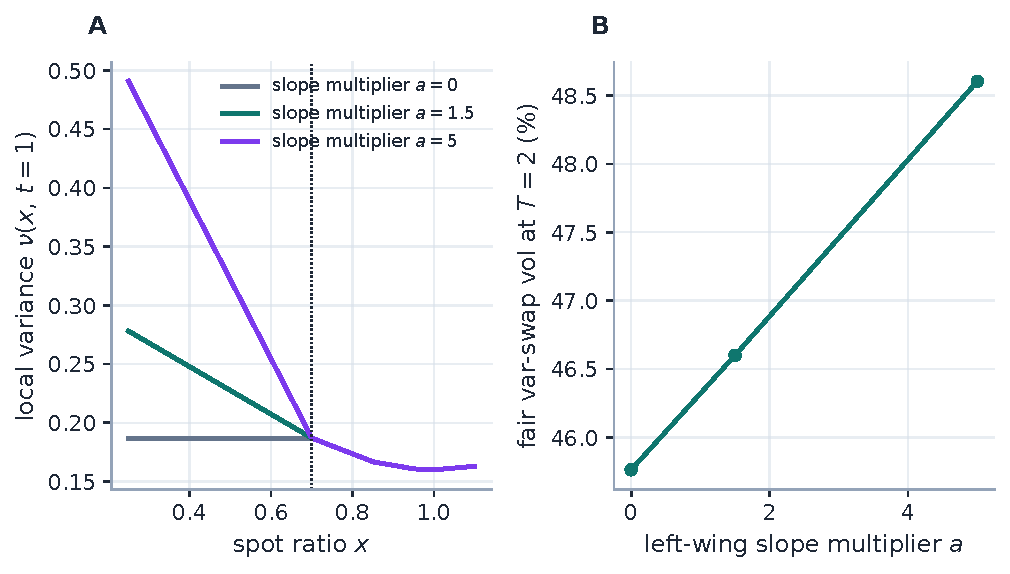
\includegraphics[width=\textwidth]{fig_wlq_lv.pdf}
\caption{The local-vol wing contract (production surface and source-PDE
pricer).  A: below the deepest strike vertex the local variance
continues linearly with slope multiplier $a$ --- a knob, not an
estimate.  B: the fair two-year var-swap strike moves by
\wlqlvswingbp\ vol bp across $a\in[0,5]$: the deep-put wing is
materially priced by the var-swap, which is exactly why $a$ becomes a
free variable only when a var-swap quote is present (Note~08).}
\label{fig:lv}
\end{figure}

\paragraph{Exercise 1.}
From the raw-SVI asymptotics $\tvar(k)\to b\big(\rho(k-m)+|k-m|\big)+a$
derive $\bL=b(1-\rho)$, $\bR=b(1+\rho)$, and hence the cap
$b(1+|\rho|)\le2$.  Verify from \cref{tab:betas} that the benchmark
fit's cap value is \wlqsvicap, and compute how much steeper the market's
put skew would have to be --- at this $b$ --- before the fence at $2$
activates.

\paragraph{Exercise 2.}
The hero slice's put slope is $\bL=\wlqherobetaL$.  Invert the Lee map
(\cref{lem:psi}) to find $q^{*}=\wlqheroqstar$: the stored SPY law has
finite moments $\E[S_T^{-q}]$ exactly up to that order.  Do the same for
the call side ($\bR=\wlqherobetaR$) and conclude that the right tail is
dramatically thinner --- then say which of the two statements a desk
should trust less, given where the quotes of \cref{fig:hero} end.

%======================================================================
\section{What has to be policed: the finite wing}
\label{sec:police}

\subsection{The limit is not the wing}

Everything so far concerned $|k|\to\infty$.  The claim that now needs
demolishing is the comfortable inference ``the slopes are admissible,
therefore the wing is fine.''  Density positivity at \emph{finite}
strike is governed not by slopes but by Durrleman's function
\begin{equation}
g(z)=\Big(1-\frac{k\,\partial_k \tvar}{2\tvar}\Big)^{2}
-\frac{(\partial_k \tvar)^{2}}{4}\Big(\frac{1}{\tvar}+\frac14\Big)
+\frac{\partial_{kk}\tvar}{2},
\label{eq:durrleman}
\end{equation}
which is proportional to the risk-neutral density at $k$
\cite{Gatheral2006}: $g\ge0$ everywhere is butterfly admissibility.
Being second-order in the smile, $g$ responds to \emph{curvature} ---
exactly what the asymptotic slope forgets.

\Cref{fig:limit} is the lecture's thesis in one exhibit, built from the
production hat kernels.  A single zero-wing hat is added to a clean
base: the realized wing slopes change by less than $10^{-16}$ (measured
at $k=\pm2.5$: \wlqhatslopediff) --- \cref{prop:zerowing} doing its job
--- while $g$ is driven to $\wlqhatgdent$ at $z=\wlqhatzmin$, deep in
the put wing, on a base whose own $g$ stays above \wlqhatbasegmin\
throughout the range.  \emph{The limit theorem is satisfied and the
smile is arbitrageable}: asymptotic admissibility and finite-range
admissibility are independent failures, and the second needs its own
police.

\begin{figure}[H]
\centering
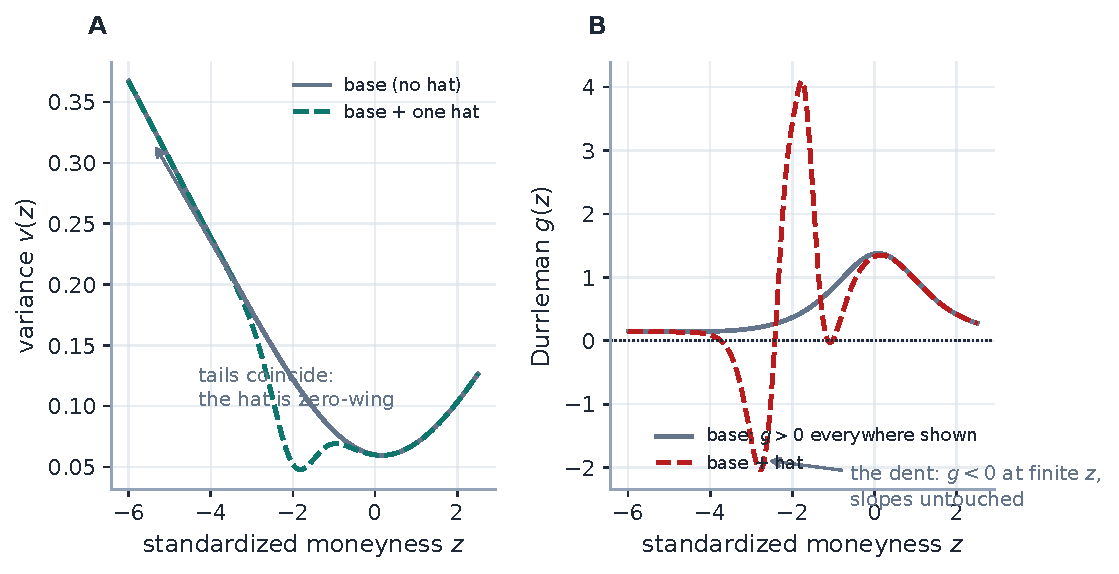
\includegraphics[width=\textwidth]{fig_wlq_limit.pdf}
\caption{The limit is not the wing (production sigmoid kernels).  A: a
single zero-wing hat added to a clean base --- the tails coincide, and
the realized wing-slope change measures below $10^{-16}$.  B: the same
hat drives Durrleman's $g$ \eqref{eq:durrleman} to \wlqhatgdent\ at
$z=\wlqhatzmin$ while the base stays positive: a butterfly arbitrage
manufactured at finite strike with the asymptotics untouched.
Admissible slopes do not make an admissible wing.}
\label{fig:limit}
\end{figure}

\paragraph{Exercise 3.}
Make the mechanism quantitative.  In standardized coordinates the last
term of \eqref{eq:durrleman} is
$\partial_{kk}\tvar/2=\partial_{zz}v/(2\sigma_{\mathrm{ref}}^{2})$.
For a hat of amplitude $\alpha<0$, width $h$ and decay $\kappa$, its
peak negative curvature scales like $|\alpha|\kappa^{2}$ (differentiate
the kernel twice).  Estimate the amplitude at which the hat of
\cref{fig:limit} ($\kappa=4$, shoulder near $z=-2.8$, base
$g\approx0.2$ there) first pushes $g$ negative, and compare with the
drawn $\alpha=-0.07$.  Conclude that hats buy \emph{local} explanatory
power at a curvature cost the asymptotic theory never sees --- which is
why their number is capped and their playground policed.

\subsection{Where the failures actually live: the census}

The backtest's arbitrage census located the MCS's finite-wing failures
precisely: $64\%$ of butterfly violations sit in the \emph{put} wing
(median worst-violation location $z\approx-3.2$), against $4\%$ at the
money --- hats fitted to sparse illiquid quotes buy in-sample RMS by
denting the density where no quote objects.  The census itself needed a
measurement lesson first: with finite-difference $g$ estimates, $28\%$
of LQD fits appeared to violate; with analytic $\partial_k\tvar,
\partial_{kk}\tvar$ per model, the LQD ``violations'' vanished entirely
(structural positivity confirmed) while the MCS ones survived ---
measure with derivatives you trust before you legislate.  (Historical
numbers throughout this subsection and the case file are quoted from
the stored backtest artifacts, never re-run; \cref{app:perf} states the
provenance.)

\subsection{The put-wing hinge}

The shipped defence has three parts, each aimed by the census:

\begin{enumerate}[leftmargin=1.6em]
\item \textbf{A capacity cap.}  The core count is clamped to $\le2$ at
the schema (and to $(n_{\mathrm{quotes}}-6)/4$ in the calibrator): most
historical violations came from high-core fits chasing noise.
\item \textbf{A one-sided Durrleman hinge.}  The refine stage carries
residual rows $\sqrt{\lambda_{\mathrm{w}}}\max(-g(z_m),0)$ on a
$49$-point grid extending \emph{two standardized units past the traded
range} on both sides, with the put side weighted $2\times$ (where the
census says the risk lives).  The weight is a declared fraction of the
$10^{3}$ base (default $100\%$).
\item \textbf{A hybrid Jacobian.}  The $g$ rows are finite-differenced,
one column at a time, while the quote/ridge/calendar blocks keep their
analytic Jacobian --- the penalty costs little and perturbs nothing when
inactive.
\end{enumerate}

\Cref{fig:hinge} shows the hinge at work on this edition's synthetic
arb slice (quotes generated by a hat-broken smile): the unpenalized
two-core fit reproduces the arbitrage at $g=\wlqarbgraw$; with the
hinge on, the fit refuses it, $g\ge\wlqarbgfixed$, conceding visible
smoothness through the pathological quotes instead.  On the clean
benchmark slice the penalty rows are identically zero and the fit is
unchanged to \wlqbyteid\ in total variance (invariant~3).  On real
illiquid wings the stored EEM result is a ${\sim}400\times$ median
repair ($-7.86\to-0.019$) at $+79$ bp of in-sample cost.

\begin{figure}[H]
\centering
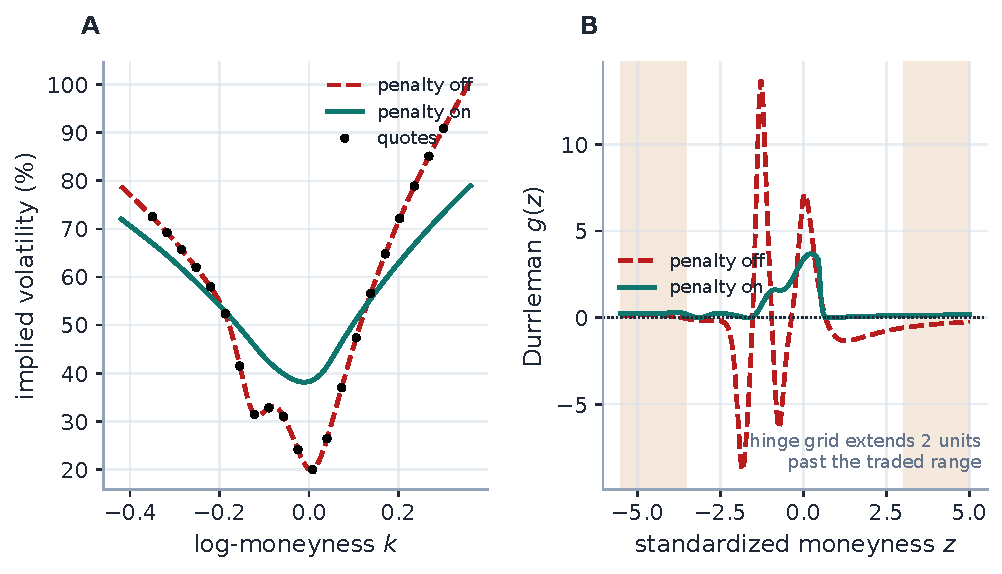
\includegraphics[width=\textwidth]{fig_wlq_hinge.pdf}
\caption{The police at work (production calibrator, synthetic arb
quotes).  A: penalty off, the two-core fit tracks every pathological
quote; penalty on, it concedes in-sample fit to stay admissible.  B: the
Durrleman view --- worst $g$ goes $\wlqarbgraw\to\wlqarbgfixed$.  The
hinge grid (shaded) deliberately extends two standardized units past the
traded range: a one-curve constraint is enforced \emph{into} the wings,
per the principle of \cref{sec:confine}.}
\label{fig:hinge}
\end{figure}

\begin{example}[title={Case file: the MCS that invented a put wing}]
\textbf{Setup.}  The three-regime backtest sweep: the Multi-Core
Sigmoid on illiquid single names, where the put wing has a handful of
wide quotes.

\textbf{Failure mode.}  The two-core fit improved in-sample RMS over
the zero-core fit --- and carried genuine butterfly arbitrage on $76\%$
of arb-prone nodes, almost all in the put wing: a hat parked where no
quote could object, buying RMS with a fake weekend wing.

\textbf{Diagnosis.}  The analytic (FD-free) arb metric separated real
violations from finite-difference noise ($28\%\to0$ for LQD ---
structural positivity confirmed --- while the MCS violations survived);
the census then localized them: put wing, $z\approx-3.2$.

\textbf{Fix.}  The two-core cap plus the put-weighted hinge above
(output side), composing with the de-Americanization convexity repair of
Note~05 (input side).

\textbf{Verdict (ablation, test-locked).}  On the arb-prone illiquid
population ($38$ census nodes, medians): with neither fix, worst $g$
$-30.4$, arbitrage on $100\%$, in-sample $92$ bp.  Input repair alone:
arbitrage cut ${\sim}3\times$ \emph{and} RMS improved to $25$ bp --- the
model had been chasing arbitraged de-Am inputs.  Output penalty alone:
arbitrage essentially eliminated ($g\ge-0.02$) but at $749$ bp ---
brutal, because the model must fight its own corrupted inputs.  Both:
the penalty's arbitrage removal at $225$ bp.  One real node makes it
concrete --- EFA in the Aug-2024 vol spike, $11$ days out, $22$ quotes:
$75$ bp at $g=-116$ with neither defence; $18$ bp but $g=-12$ with the
repair alone; arb-free at $726$ bp with the penalty alone; arb-free at
$34$ bp with both.  \emph{Complementary, not redundant: the input
repair makes the output penalty affordable.}  On liquid names both are
byte-identical no-ops.
\end{example}

%======================================================================
\section{Where constraints have jurisdiction: the confinement principle}
\label{sec:confine}

The hinge of \cref{sec:police} is enforced \emph{past} the quoted range;
the calendar floor of Note~10 is enforced \emph{only inside} it.  Both
choices are correct, and four production incidents --- the phantom
calendar violations (Note~10's case file), the local-vol convex-wing
regression (Note~04), the de-Am global-repair revert (Note~05), and the
put-wing penalty above --- resolve into one rule for telling them apart.

\begin{heuristic}
\textbf{The confinement principle.}  \emph{A constraint that compares
two curves must be sampled only where data pins both; a constraint
intrinsic to one curve must hold everywhere, wings included.}  A
two-curve constraint evaluated where both sides are extrapolation can
only compare two fictions --- any ``violation'' there is an artefact of
the extrapolation laws, and enforcing it lets the fiction corrupt the
fit where data \emph{does} live.  A single-curve constraint (density
positivity, call convexity) is a property of the law itself: it has no
rival extrapolation to be spuriously violated against, and abandoning it
in the wings is exactly how fake tails are born.
\end{heuristic}

\Cref{fig:confine} manufactures the two-curve failure from two clean
production fits.  A steep short slice and a flatter long slice satisfy
the calendar order everywhere the data lives: sampled on the confined
floor grid, the worst violation is \wlqphantominside\ variance bp ---
none.  Sampled on a wide grid running to $|k|=1$, the two
\emph{extrapolations} cross and a phantom violation of
\wlqphantomwide\ variance bp appears --- between two curves, at strikes
where neither has ever seen a quote.  Enforcing it would bend both fits
where the data does live to fix a disagreement between fictions; the
production floor grid is confined to the observed span for exactly this
reason.

\begin{figure}[H]
\centering
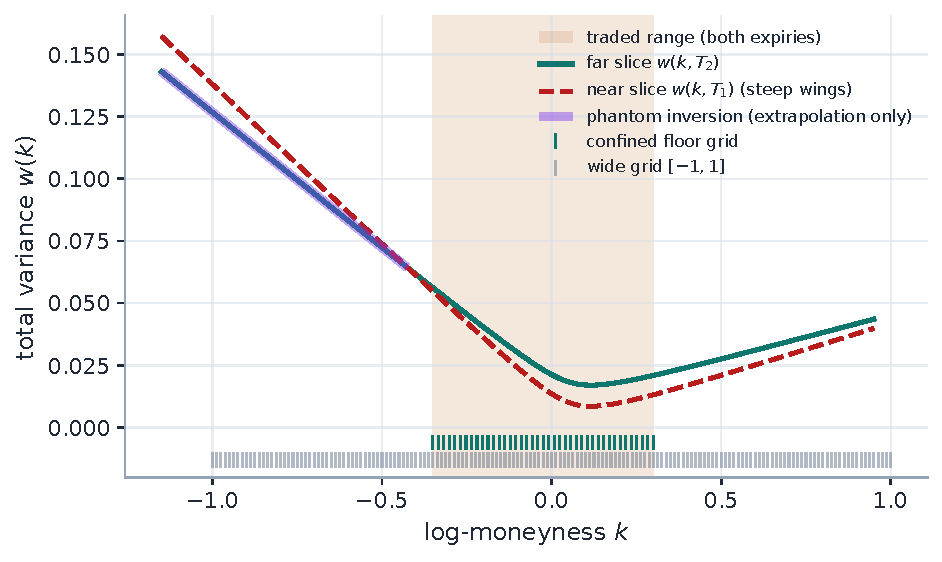
\includegraphics[width=0.88\textwidth]{fig_wlq_confine.pdf}
\caption{The phantom a wide grid manufactures (two clean production SVI
fits).  Inside the traded range the calendar order
$\tvar(k,T_2)\ge \tvar(k,T_1)$ holds with margin (worst violation
\wlqphantominside\ bp).  In the extrapolated region the near slice's
steeper stated wing overtakes the far slice's --- a
\wlqphantomwide-variance-bp ``violation'' between two fictions
(highlighted), visible only to the wide sampling grid (lower ticks).
The production floor grid (upper ticks) is confined to the data span:
two-curve constraints have no jurisdiction where neither curve is
pinned.}
\label{fig:confine}
\end{figure}

\begin{center}
\small
\begin{tabular}{p{0.30\textwidth}p{0.13\textwidth}p{0.22\textwidth}p{0.24\textwidth}}
\toprule
Constraint & Curves & Treatment & Where\\
\midrule
Calendar floor $\tvar_{\mathrm{far}}\ge \tvar_{\mathrm{near}}$ & two &
\textbf{confined} to traded range & Note~10\\
LV convex-wing hinge & two\footnotemark & \textbf{confined} to the
extrapolation tail below the deepest quote & Note~04\\
MCS Durrleman $g\ge0$ & one & \textbf{extended} $\pm2$ ATM-std past
quotes & \cref{sec:police}\\
De-Am call convexity & one & \textbf{extended} to the wings, but
band-constrained and ATM-core-fixed & Note~05\\
\bottomrule
\end{tabular}
\end{center}
\footnotetext{The LV wing hinge compares the model's wing against the
\emph{quotes'} implied shape when sampled inside the quoted range ---
the regression of Note~04 --- so it behaves as a two-curve constraint
and is confined; in the pure extrapolation tail it degenerates to a
one-curve convexity preference, which is where it is allowed to act.}

The de-Am row is the principle's refinement rather than an exception:
the \emph{constraint} (convexity, one-curve) rightly extends into the
wings, but the \emph{repair} it licenses is confined --- to the quoted
bid--ask band and away from the ATM core --- because a repair, unlike a
constraint, moves prices.  Extending a one-curve constraint is safe;
extending a repair's \emph{authority} unboundedly is how a $27\%$ put
wing became $104\%$ (Note~05).

\begin{remark}[Open problem: softer two-curve enforcement in the wings]
\label{rem:softwings}
Confinement as stated is binary: a two-curve constraint is either
sampled (inside the traded range) or ignored (outside).  But the
extrapolated region is not uniformly worthless --- just past the last
quote the options still carry genuine premium, and there a calendar
inversion between two \emph{stated} wing contracts (\cref{sec:choose})
is a real inconsistency even if no quote witnesses it.  Whether
two-curve constraints deserve \emph{softer} enforcement in the
near-extrapolation region --- weight decaying with distance past the
last quote, or with remaining time value --- is open (flagged 2026-07),
to be settled jointly with Note~10's floor-grid construction.  Three
production phases already frame it: Phase~1, the Quality report
\emph{measures} the region (worst Durrleman $g$, calendar crossings and
wing-slope order over the time-value envelope), advisory only, never
gating readiness.  Phase~2, an opt-in tapered enforcement (off by
default) adds exactly those three hinges to the SVI/MCS overlay fits,
budgeted in vol units at a fraction of the data weight so it leans
without outvoting quotes; the far-field calendar order is enforced
through the \emph{scalar} wing-slope condition, never pointwise.
Phase~3, a publish-time wing-only projection lifts exported curve
samples onto the discrete arbitrage-free cone in OTM-price space, traded
core pinned byte-identically, fits and in-app views untouched --- a
repair, so its \emph{authority} is confined to the wings even though the
constraints it restores extend there.  Note~10's matching remark
carries the mechanism and the measured lean/cost trade.
\end{remark}

%======================================================================
\section{What is genuinely original here}
\label{sec:original}

The Lee theory is classical; the contributions are structural.
\begin{enumerate}[leftmargin=1.6em]
\item The \emph{prove/choose/police division} as an engineering
discipline: the same slope $\beta$ is computed three structurally
different ways (\eqref{eq:lqd_wings}, the SVI closed forms,
\eqref{eq:siv_wings}) and shown to agree in ordering on one window, so
model choice is a choice of \emph{how} to extrapolate, never
\emph{whether} the extrapolation is admissible --- and each model's
contract states which of the three verbs guards it (structural / capped
/ diagnosed / knob).
\item The \emph{census-guided} put-wing regularizer: placed where the
measured violations live, weighted by their measured asymmetry, and
validated by an ablation that also proved it composes with the
input-side repair rather than duplicating it.
\item The \emph{confinement principle} with its two-curve/one-curve
criterion --- four hard-won production incidents compressed into one
transferable design rule, exhibited here (\cref{fig:confine}) as a
measured phantom rather than an anecdote.
\end{enumerate}

%======================================================================
\section{Limitations}
\label{sec:limits}

Where the guarantees stop.  \emph{MCS base admissibility is diagnosed,
not enforced}: \cref{prop:zerowing} protects the wings from the hats,
but nothing bounds the base slopes into the Lee cone --- the diagnosis
lives in the quality report, not the optimizer.  \emph{The ceiling is
open at the top} (\cref{rem:boundary}): a model pinned exactly at
$\beta=2$ is already wrong, which is why the LQD barrier keeps
$\AR<1$ strictly and the SVI cap is a fence, not a target.  \emph{The
historical numbers are population-specific}: the census asymmetry
($64\%$ put wing) and the ablation grid were measured on the illiquid
single-name population of one backtest campaign; the hinge's put-side
$2\times$ weighting hard-codes that asymmetry until a new census says
otherwise.  \emph{The hero share is a display statement}:
\wlqheroextrapshare\% quantifies the drawn curve, whose strike range is
itself a UI choice --- the economically weighted share (by time value or
var-swap mass, Note~08) is smaller but still material.  \emph{The
hinge's Jacobian is hybrid}: the $49$ finite-differenced rows are cheap,
but a fully analytic $g$-row Jacobian remains undone.  And
\emph{confinement is binary} (\cref{rem:softwings}): the
near-extrapolation region --- real premium, no quotes --- currently gets
measurement (Phase~1) and opt-in leaning (Phase~2), not settled
doctrine.

\appendix
%======================================================================
\section{Hyperparameter atlas}
\label{app:atlas}

The only home for settings names: the body speaks mathematics, this
table speaks configuration.

\begin{longtable}{p{0.27\textwidth}p{0.13\textwidth}p{0.51\textwidth}}
\caption{Wing-related knobs (cross-model).}\label{tab:atlas}\\
\toprule Knob & Default & Role\\ \midrule
\endfirsthead \toprule Knob & Default & Role\\ \midrule \endhead
\multicolumn{3}{l}{\emph{Surfaced}}\\ \midrule
\texttt{sivWingPenaltyPct} & $100$ & Put-wing Durrleman hinge strength
(\% of the $10^{3}$ base weight); $0$ disables.\\
\texttt{nCores} & $2$ (max $2$) & MCS core count, schema-clamped
(\cref{sec:police}).\\
\texttt{leeSlopeMax} & $2.0$ & SVI Lee cap $b(1+|\rho|)\le\beta_{\max}$.\\
\texttt{sviPenaltyWeight} & $10^{3}$ & Weight of the SVI Lee /
min-variance hinges.\\
\texttt{leftWingSlopeMult} & $1.5$ & LV left extrapolation slope seed;
free variable (box $[0,20]$) under a var-swap quote.\\
\texttt{lvVolCapMult} & $3.0$ & LV local-vol cap multiple (Note~04).\\
\texttt{convexWing} & \texttt{false} & LV convex-wing hinge, confined to
the $5\Delta$ tail beyond the deepest quote.\\
\texttt{extrapEnforce} & \texttt{false} & Phase-2 tapered
extrapolated-region hinges (\cref{rem:softwings}).\\
\midrule
\multicolumn{3}{l}{\emph{Hidden}}\\ \midrule
\texttt{\_WING\_PAD} & $2.0$ & The $g$-grid extends $\pm2$ standardized
units past the traded range.\\
\texttt{\_WING\_GRID} & $49$ & Points on the $g$-grid.\\
\texttt{\_WING\_PUT\_FACTOR} & $2.0$ & Extra weight on the put side
(the census asymmetry).\\
\texttt{EPS\_AR} & $10^{-6}$ & LQD $\AR<1$ buffer; the only LQD wing
constraint (Note~01, \cref{rem:boundary}).\\
\texttt{VAR\_FLOOR\_N\_DATA} & $41$ & Points of the confined calendar
floor grid (traded span); the wide diagnostic grid is $161$ points on
$[-1,1]$.\\
\bottomrule
\end{longtable}

%======================================================================
\section{Performance notes}
\label{app:perf}

Protocol: fresh numbers in this edition (slopes, hinge repair,
byte-identity, phantom sizes, the LV var-swap swing) are produced by the
generator running production code; historical backtest numbers (the
census shares and location, the $28\%\to0$ analytic-metric episode, the
EEM $400\times$ repair, the ablation grid $92/25/749/225$ bp and the
EFA node) are quoted from the stored artifacts
\texttt{backend/backtest/FINDINGS\_calibration\_arb.md},
\texttt{FINDINGS\_ablation\_arb.md} and
\texttt{results/spike\_aug2024\_ablation\_arb\_EEM\_EFA\_2d.json}, and
are never re-run by a documentation build.

\begin{enumerate}[leftmargin=1.6em]
\item Wing handling is essentially free: LQD slopes are a by-product of
the endpoint scales; SVI/MCS slopes are closed forms of fitted
parameters; the LV wing is part of the surface solve.
\item The put-wing hinge adds $49$ residual rows in the refine stage
only, with a hybrid Jacobian (analytic blocks untouched, $g$ rows by
central differences); on a clean slice the rows are zero and the
optimum is unchanged to \wlqbyteid.
\item The analytic arb metric replaced a double \texttt{np.gradient} on
$201$ points with closed-form $\partial_k\tvar,\partial_{kk}\tvar$ per
model --- more accurate \emph{and} cheaper; it is what made the census
trustworthy (\cref{sec:police}).
\item Confinement reduces work by not over-constraining the
extrapolation region: the floor grid is $41$ points on the data span
instead of $161$ on $[-1,1]$.
\item The stable $\psi$ evaluation (\cref{rem:naive}) costs one extra
division and removes an entire class of underflow misreads at extreme
endpoint scales.
\end{enumerate}

%======================================================================
\section{Traceability}
\label{app:trace}

\begingroup
\small
\setlength{\tabcolsep}{4pt}
\renewcommand{\arraystretch}{1.15}
\begin{longtable}{@{}p{0.42\textwidth}p{0.10\textwidth}p{0.44\textwidth}@{}}
\caption{Claims in this note and the code/tests that lock them.}
\label{tab:trace}\\
\toprule Claim & Object & Code anchor \newline \emph{Test anchor}\\ \midrule
\endfirsthead
\toprule Claim & Object & Code anchor \newline \emph{Test anchor}\\ \midrule
\endhead
LQD structural Lee slopes; underflow-safe &
\eqref{eq:lqd_wings} &
\nolinkurl{volfit/models/lqd/basis.py}\newline
\nolinkurl{tests/test_lqd_basis.py::test_svi_fit_lee_slopes_match_note};
\nolinkurl{::test_lee_slopes_handle_underflowed_endpoint_scales}\\
\addlinespace
SVI Lee cap enforced &
\cref{sec:choose} &
\nolinkurl{volfit/models/svi_jw/calibrate.py}\newline
\nolinkurl{tests/test_svi_calibrate.py::test_respects_lee_wing_bound}\\
\addlinespace
MCS hats are zero-wing &
\cref{prop:zerowing} &
\nolinkurl{volfit/models/sigmoid/sigmoid.py},
\nolinkurl{kernels.py}\newline
\nolinkurl{tests/test_sigmoid_model.py}\\
\addlinespace
Two-core cap (schema and calibrator) &
\cref{sec:police} &
\nolinkurl{volfit/api/schemas.py},
\nolinkurl{volfit/models/sigmoid/calibrate.py}\newline
\nolinkurl{tests/test_siv_wing_penalty.py::test_cores_clamped_to_two}\\
\addlinespace
Put-wing hinge removes wing arb; byte-identical on clean slices &
\cref{fig:hinge} &
\nolinkurl{volfit/models/sigmoid/calibrate.py}\newline
\nolinkurl{tests/test_siv_wing_penalty.py::test_penalty_removes_wing_arb};
\nolinkurl{::test_penalty_byte_identical_on_arb_free_slice}\\
\addlinespace
Analytic FD-free arb metric &
\cref{sec:police} &
\nolinkurl{backend/backtest/dispatch.py},
\nolinkurl{volfit/models/sigmoid/kernels.py}\newline
\nolinkurl{tests/test_backtest_arb.py}\\
\addlinespace
Input/output ablation: complementary &
case file &
\nolinkurl{backend/backtest/ablation_arb.py}\newline
\nolinkurl{tests/test_ablation_arb.py}\\
\addlinespace
De-Am wing repair (input side; confined authority) &
\cref{sec:confine} &
\nolinkurl{volfit/calib/convex_deam.py}\newline
\nolinkurl{tests/test_convex_deam.py}\\
\addlinespace
Calendar floor confined (two-curve) &
\cref{fig:confine} &
\nolinkurl{volfit/calib/calendar.py}\newline
\nolinkurl{tests/test_overlay_calendar.py::test_wide_grid_breaks_svi_but_data_grid_does_not}\\
\addlinespace
LV convex wing confined to the tail &
\cref{sec:confine} &
\nolinkurl{volfit/api/affine_fit.py}\newline
\nolinkurl{tests/test_affine_grid_design.py::test_convex_wing_confined_to_quoted_extrapolation}\\
\bottomrule
\end{longtable}
\endgroup

%======================================================================
\section{Reference implementation: the Lee maps}
\label{app:ref}

Both listings were executed against their production counterparts by
this edition's generator on every run: $\psi$ over
$p\in[10^{-4},50]$ and the slopes on the benchmark fit agree to
\wlqrefagree\ (floating-point identity).  The $\psi$ listing is the
production \emph{stable} form of \cref{rem:naive} --- the naive
textbook expression is reproduced only to exhibit its failure
($\wlqnaivepsi$ at $p=10^{16}$).

\begin{lstlisting}[caption={Lee's $\psi$ (stable form) and the LQD
structural wing slopes from the endpoint scales (distilled from
\texttt{models/lqd/basis.py}).},label={lst:lee}]
def lee_psi(p):                    # beta = psi(p); decreasing, psi(0) = 2
    return 2.0 - 4.0 / (np.sqrt(1.0 + 1.0/p) + 1.0)   # no cancellation

def lee_slopes(A_L, A_R):          # exponential tails -> exact exponents
    beta_L = lee_psi(1.0/A_L) if A_L > 0 else 0.0     # left:  q* = 1/A_L
    if A_R >= 1.0:                                    # ceiling guard
        return beta_L, 2.0
    beta_R = lee_psi(1.0/A_R - 1.0) if A_R > 0 else 0.0  # right: p* = 1/A_R - 1
    return beta_L, beta_R
\end{lstlisting}

\begin{thebibliography}{9}
\bibitem{Lee2004} R.~W.~Lee.  The moment formula for implied volatility
at extreme strikes.  \emph{Mathematical Finance}, 14(3):469--480, 2004.
\bibitem{BenaimFriz2009} S.~Benaim and P.~Friz.  Regular variation and
smile asymptotics.  \emph{Mathematical Finance}, 19(1):1--12, 2009.
\bibitem{Gatheral2006} J.~Gatheral.  \emph{The Volatility Surface}.
Wiley, 2006.  (The density factor $g$.)
\bibitem{GatheralJacquier2014} J.~Gatheral and A.~Jacquier.
Arbitrage-free SVI volatility surfaces.  \emph{Quantitative Finance},
14(1):59--71, 2014.
\end{thebibliography}

\end{document}
